\section{Exploración Dimensión del Cromosoma}

\begin{table}[]
    \centering
    \begin{tabular}{||c|c|c|c|c|c||}
        \hline
        \textbf{Fichero Configuración} & \textbf{Generaciones} & \textbf{DIM} & \textbf{Tmñ. poblacion} & \textbf{Mejor fitness} & \textbf{Evals. de f}\\ \hline
        Config 10  & 45   & 10    & 1000   & -38.48    &  69537    \\ \hline
        Config 11  & 92   & 15    & 1500   & -38.88    &  211163   \\ \hline
        Config 12  & 62   & 30    & 3000   & 79.74     &  288787   \\ \hline
        Config 13  & 78   & 50    & 5000   & 346.941   &  602536   \\ \hline
        Config 14  & 94   & 100   & 10000  & 1266.01   &  1459146  \\ \hline
    \end{tabular}
    \caption{Resultados exploración inicial}
    \label{tab:exploracion_dim_cromosoma}
\end{table}

Para realizar esta exploración se ha seguido el mismo proceso que en las anteriores. El algoritmo se ha ejecutado 15 veces por cada fichero de configuración.
Se toma como base el tamaño de población 1000, que irá variando proporcionalmente a la dimensión del cromosoma. El resumen de estas ejecuciones está en la 
Tabla \ref{tab:exploracion_dim_cromosoma}. 

\begin{figure}[]
	\centering	
	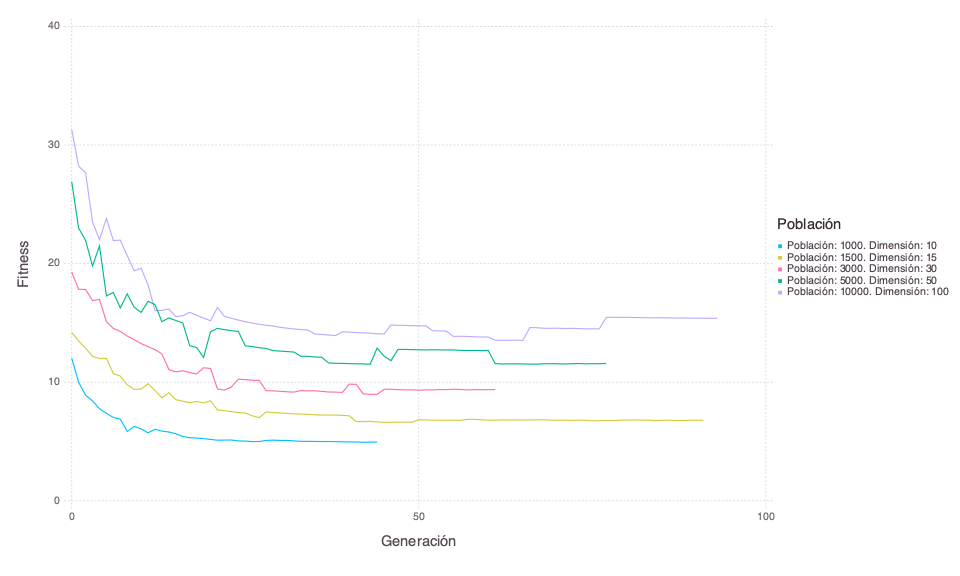
\includegraphics[scale=0.5]{figuras/ps_cd_variation.png}
	\caption{ Variación del fitness a lo largo de las generaciones }
    \label{fig:exec_summary}
\end{figure}

\begin{figure}[]
	\centering	
	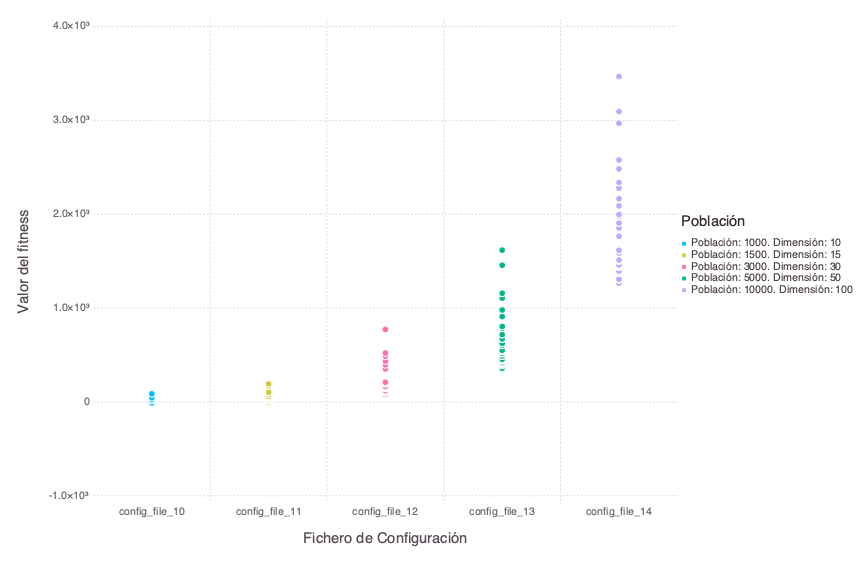
\includegraphics[scale=0.5]{figuras/ps_cd_point.png}
	\caption{ Variación de los resultados, variando la dimensión del cromosoma }
    \label{fig:box_plots_crom_dim}
\end{figure}

Viendo la Figura \ref{fig:exec_summary}, todas las ejecuciones tienen un comportamiento parecido, gran descenso del valor del fitness al principio y estancamiento al final. 
En la decisión final se descartan las 2 primeras configuraciones, ya que la exploración que hacen es pequeña y aun así consiguen un buen valor de fitness. Por tanto
no nos interesa a la hora de escoger la dimensión del cromosoma, ya que queremos elegir uno que explore bien el espacio de búsqueda y así mantenga la diversidad.
Una conclusión. Se elige, por tanto la configuración 13, ya que tiene un espacio de búsqueda mayor que las anteriores y no se aleja mucho de la solución.